%% ------------------------------------------------------------------------
%% Copyright (C) 2021,2022 SJTUG
%% 
%% SJTUBeamer 快速入门
%% 
%% SJTUBeamear 符合 Apache-2.0 开源许可,不提供任何担保。
%% sjtuvi.sty 和 sjtucover.sty 库及其附属徽标、图片不符合上述开源许可,
%% 由上海交通大学持有版权。
%% 详细许可证信息参见 SJTUBeamer 存储库:https://github.com/sjtug/SJTUBeamer
%% -----------------------------------------------------------------------

% 本行为文件元数据,可省略。
\ProvidesFile{sjtubeamerquickstart.tex}[2022/11/23 v3.0.0 Quick Start for sjtubeamer (Chinese)]

% 加载 ctexbeamer 文档类【第一部分】
% 如果编写英文内容,建议直接使用 beamer 文档类。
\documentclass[
    % draft,          % 草稿模式
    aspectratio=169,  % 使用 16:9 比例
]{ctexbeamer}

% 演示模式(可选)
\mode<presentation>

% 加载 SJTUBeamer 主题【第二部分】
\usetheme[maxplus,default]{sjtubeamer}
% 使用 maxplus/max/min 切换标题页样式
% 使用 red/blue 切换主色调
% 使用 light/dark 切换亮/暗色模式
% 使用外样式关键词以获得不同的边栏样式
%   miniframes infolines  sidebar 
%   default    smoothbars split	 
%   shadow     tree       smoothtree
% 使用 topright/bottomright 切换徽标位置

% 加载插件(可选)【第三部分】
% 当前目录下需要有 contrib 文件夹。
% \usesjtutheme{sjtug}

% \tikzexternalize[prefix=build/]
% 如果您需要缓存 tikz 图像,请取消注释上一行,并在编译选项中添加 -shell-escape。

% 引用设置
\usepackage[backend=biber,style=gb7714-2015]{biblatex}
\addbibresource{ref.bib}

% 其他宏包
\usepackage{multicol}
\usepackage{pgfplots}
\usepackage{pgfplotstable}
\usepackage[ruled, linesnumbered]{algorithm2e}

% 使用节目录
% 还可以通过 \AtBeginSubsection[]{} 设置小节目录
\AtBeginSection[]{
  \begin{frame}
    % 传统节目录,使用了印记标记设计
    % \tableofcontents[currentsection,hideallsubsections]
    % 节页,使用了专门设计的节次页
    \sectionpage
  \end{frame}
}

% 标题
\title{SJTUBeamer 幻灯片模板 快速入门}
% 副标题
\subtitle{SJTUBeamer Template Quick Start}
% 作者
\author{SJTUG}
% 组织
\institute[Linux User Group]{Linux 用户组}
% 日期
\date{\today}

% 文档开始
\begin{document}

% 创建标题页
\maketitle

% 创建新页(无标题)
\begin{frame}
  % 创建列表
  \begin{itemize}
    \item 欢迎使用 SJTUBeamer!SJTUBeamer 是上海交通大学的非官方 \LaTeX{} Beamer 幻灯片模板。

    \item 如果你手上已经有 \LaTeX{} 手稿,使用 \texttt{beamer} 文档类 \footfullcite{beamerman}
          可以借助于原生 \LaTeX{} 的排版能力快速完成一份高质量学术幻灯片。

    \item 而 SJTUBeamer 借助于 \texttt{ctexbeamer} 文档类 \footfullcite{ctex} 提供的中文适配,
          参考上海交通大学视觉形象系统 \footfullcite{viman},提供用户友好的命令接口编写具有交大特色
          的幻灯片。

    \item 本页为第 2 页,在此之前已经有很多设置代码,请对照源代码及其注释观察编译结果以快速上手。
  \end{itemize}
\end{frame}

% 创建部分
% SJTUBeamer 会自动为部分起始位置添加部分页。
% 对于本幻灯片设置部分这一级可能不太必要,最好在长文档(每章超过 20 页)的文档使用部分这一级。
% 注意,beamer 不设置 chapter 这一级。
\part{beamer 简要入门}

\begin{frame}
  % 页标题
  % \begin{frame}{<title>} 的用法属于老式用法,在一些情况下可能会有问题。
  \frametitle{文档结构}
  % 页子标题
  \framesubtitle{一篇幻灯片的整体结构}

  \begin{enumerate}
    \item \texttt{beamer} 文档类将整个文档组织成多个 \texttt{frame} 环境。
    \item 典型的幻灯片排版方式是按点排列,可以在 \texttt{frame} 内使用 \texttt{itemize},
          \texttt{enumerate}, \texttt{description} 环境安排内容要点。
    \item \texttt{frame} 内支持覆盖(overlay),一帧可以通过像 \texttt{<1>} 的覆盖参数生成
          多页幻灯片。
    \item \texttt{frame} 内页支持使用 \texttt{columns} 环境分割多栏,更多信息参见
          \texttt{beamer} 用户手册\cite{beamerman}。
  \end{enumerate}

\end{frame}

\begin{frame}
  \frametitle{盒子}
  \framesubtitle{强调内容}

  % 创建盒子时标题参数不可省略,如果不需要标题,也需要留一个空参数 {}
  \begin{block}{盒子}
    普通盒子
  \end{block}
  \begin{alertblock}{注意}
    注意内容
  \end{alertblock}
  \begin{exampleblock}{示例}
    示例内容
  \end{exampleblock}
\end{frame}

\begin{frame}
  \frametitle{\LaTeX{} 原生}
  \framesubtitle{发挥 \LaTeX{} 的特长}

  % 使用 align 环境对齐公式,带星号为无编号环境
  \begin{align*}
    \mathnormal{e}^x & = 1+x+\frac{x^{2}}{2!}+\frac{x^{3}}{3!}+\cdots+\frac{x^{n}}{n!}+\cdots                    \\
    \ln (1+x)        & = x-\frac{x^{2}}{2}+\frac{x^{3}}{3}-\frac{x^{4}}{4}+\cdots+(-1)^{n-1}\frac{x^n}{n}+\cdots \\
  \end{align*}

  % 使用 theorem 等内置环境创建定理块,中括号内的可选参数为定理标题
  \begin{theorem}[Chebyshev 不等式]
    设随机变量 $X$ 具有数学期望 $E(X)=\mu$,方差 $D(X)=\sigma^2$,则对于任意整数
    $\epsilon$,恒有不等式
    \begin{equation}
      P\left(\lvert X-\mu\rvert<\epsilon\right)>1-\frac{\sigma^2}{\epsilon^2}
    \end{equation}
  \end{theorem}

\end{frame}

\part{SJTUBeamer 独有内容}

\begin{frame}
  \frametitle{提纲}
  % 创建该部分的目录。
  \tableofcontents
\end{frame}

\section{多种样式}

\begin{frame}
  \frametitle{切换样式}
  \framesubtitle{封面页、节次页、结束页与外样式}

  SJTUBeamer 提供了丰富的样式选择,更改载入选项以切换设计样式。

  % 多栏环境,使用 T 顶部对齐
  \begin{columns}[T]
    % 栏环境,用于手动创建不同的竖栏
    \begin{column}{0.22\textwidth}
      \begin{alertblock}{子主题}
        \ttfamily
        \begin{itemize}
          \item maxplus
          \item max
          \item min
          \item my
        \end{itemize}
      \end{alertblock}
      \begin{block}{插件}
        \ttfamily
        \begin{itemize}
          \item sjtug
          \item $\cdots$
        \end{itemize}
      \end{block}
    \end{column}
    \begin{column}{0.7\textwidth}
      \begin{columns}[t]
        \begin{column}{0.25\textwidth}
          \begin{alertblock}{色调}
            \ttfamily
            \begin{itemize}
              \item red
              \item blue
            \end{itemize}
          \end{alertblock}
        \end{column}
        \begin{column}{0.25\textwidth}
          \begin{alertblock}{亮度}
            \ttfamily
            \begin{itemize}
              \item dark
              \item light
            \end{itemize}
          \end{alertblock}
        \end{column}
        \begin{column}{0.3\textwidth}
          \begin{alertblock}{徽标位置}
            \ttfamily
            \begin{itemize}
              \item topright
              \item bottomright
            \end{itemize}
          \end{alertblock}
        \end{column}
      \end{columns}
      \begin{alertblock}{外样式}
        \ttfamily
        % 也可以使用 multicols 环境自动分割多栏
        \begin{multicols}{3}
          \begin{itemize}
            \item miniframes
            \item infolines
            \item sidebar
            \item default
            \item smoothbars
            \item split
            \item shadow
            \item tree
            \item smoothtree
          \end{itemize}
        \end{multicols}
      \end{alertblock}
    \end{column}
  \end{columns}
\end{frame}

\section{专用区块}

\begin{frame}
  \frametitle{强调内容}

  % \paragraph{段落标题}
  \paragraph{小段} SJTUBeamer 可以使用普通的分段命令强调段落标题。

  % \highlight<覆盖参数>[颜色]{高亮文字}
  \highlight{高亮} SJTUBeamer 提供高亮命令用主题色高亮文本。

  % \stamptext[颜色]{文字}
  \stamptext{注} SJTUBeamer 提供印记形文字块。

  % \stamphrule[颜色] 创建分割线。
  \stamphrule

  \begin{columns}
    \begin{column}{0.4\textwidth}
      % \begin{stampblock}<覆盖参数>[编号]{文字}
      \begin{stampblock}{印记区块标题}
        印记区块内容。
      \end{stampblock}
    \end{column}
    \begin{column}{0.3\textwidth}
      % \begin{stampbox}[颜色] 创建印记边框盒子。
      \begin{stampbox}
        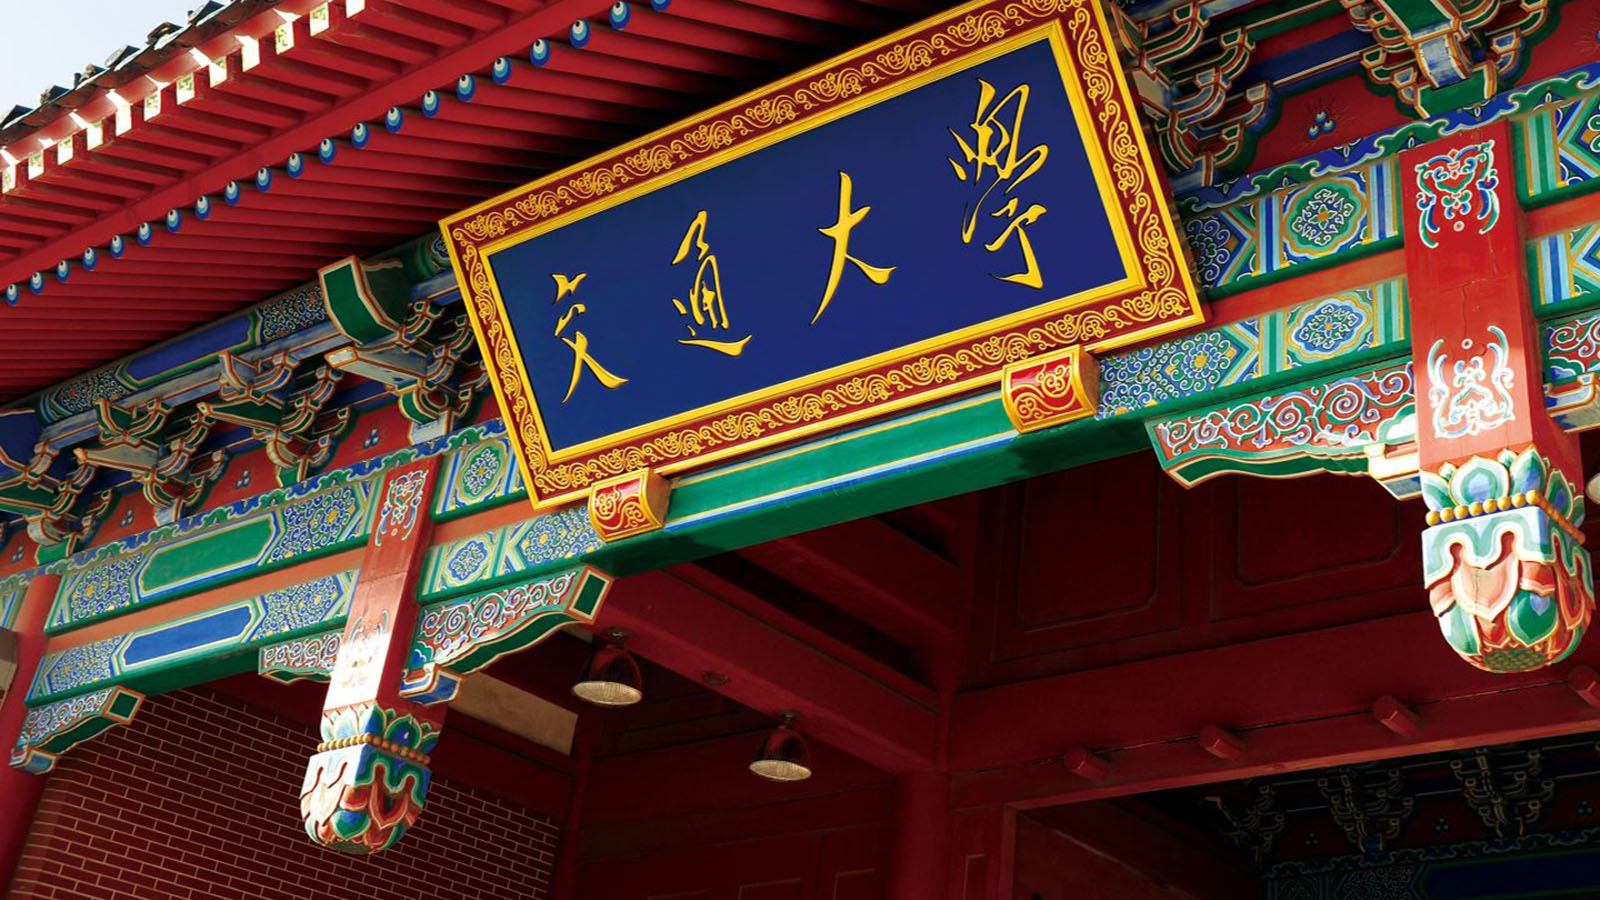
\includegraphics[width=0.9\textwidth]{vi/sjtuphoto.jpg}
      \end{stampbox}
    \end{column}
    \begin{column}{0.3\textwidth}
      \begin{tikzpicture}
        % \stamparray{单体半宽}{起始点}{终止点} 用于创建印记矩阵。
        \stamparray{16pt}{(0,0)}{(4,3)}
      \end{tikzpicture}
    \end{column}
  \end{columns}

\end{frame}

% 当该帧内有代码抄录时,fragile 参数是必需的。
\begin{frame}[fragile]
  \frametitle{代码抄录}

  % \begin{codeblock}[listing 参数]{标题} 创建代码块
  % \highlightline<覆盖参数> 用于高亮当前行
  \begin{codeblock}[language=c++,escapechar=|]{C++代码}
#include<iostream>

int main(){
  // Console Output
  std::cout << "Hello, SJTU!" << std::endl;
|\highlightline|  return 0;
}
  \end{codeblock}
\end{frame}

\section{宏包优化}

\begin{frame}
  \frametitle{图表}
  \framesubtitle{\texttt{pgfplots}, \texttt{pgfplotstable}}

  % SJTUBeamer 对 pgfplots 和 pgfplotstable 进行了优化,
  % 引用宏包以启用之。
  \begin{columns}[T]
    \begin{column}{0.6\textwidth}
      \begin{figure}
        \caption{平均时间趋势图}\label{fig:avgtime}
        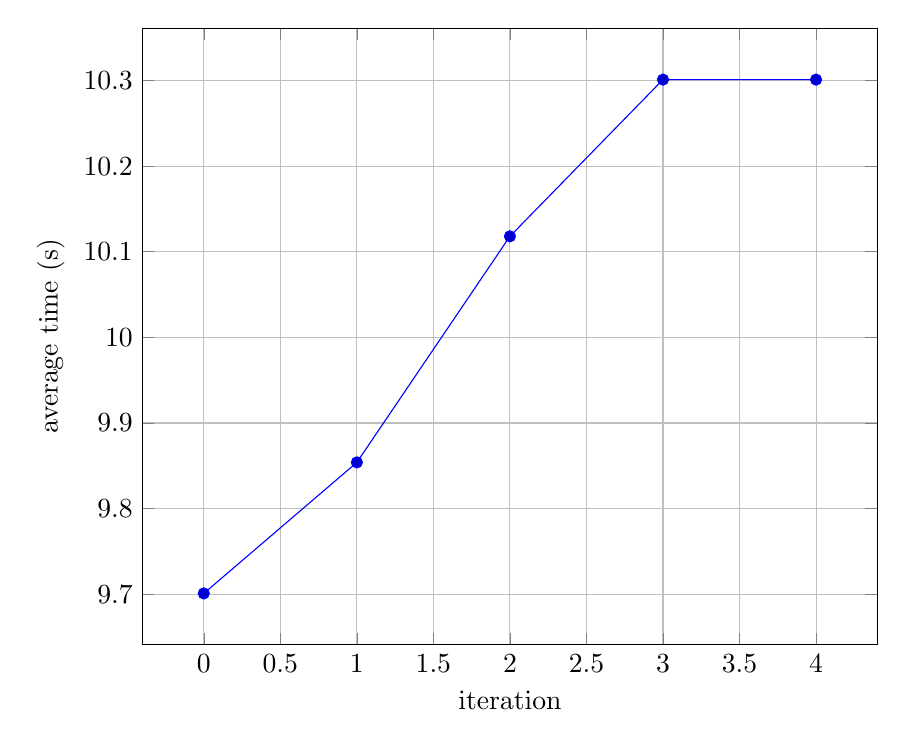
\begin{tikzpicture}
          % SJTUBeamer 内置了一些统计图上颜色的优化。
          \begin{axis}[
              xlabel={iteration},
              ylabel={average time (s)},
              width=0.9\textwidth,
              grid=major
            ]
            \addplot+ coordinates {
                (0,9.701) (1,9.854)
                (2,10.118) (3,10.301)
                (4,10.301)
              };
          \end{axis}
        \end{tikzpicture}
      \end{figure}
    \end{column}
    \begin{column}{0.4\textwidth}
      \begin{table}
        \caption{平均时间变化表}\label{tab:avgtime}
        % SJTUBeamer 将表格设定为三线表样式。
        % 也可以在第二个参数里使用现有的 csv 文件,
        % 使用文件时,请不要设定 col sep 和 row sep 参数。
        % 比如:\pgfplotstabletypeset[]{test.csv}
        \pgfplotstabletypeset[
        col sep=&, row sep=\\,
        columns/average time (s)/.style={
        fixed, dec sep align, fixed zerofill, precision=3
        }
        ]{
        iteration & average time (s)\\
        0         & 9.701           \\
        1         & 9.854           \\
        2         & 10.118          \\
        3         & 10.301          \\
        4         & 10.301          \\
        }
      \end{table}
    \end{column}
  \end{columns}
\end{frame}

\begin{frame}
  \frametitle{算法块}
  \framesubtitle{\texttt{algorithm2e}}

  % SJTUBeamer 将 algorithm2e 宏包的 Algorithm 1 翻译为 算法 1。
  % 浮动体参数 [H] 不可忽略。
  \begin{algorithm}[H]
    \caption{冒泡排序}\label{alg:bubblesort}
    \KwIn{含有 $n$ 个元素的数组 $A$}
    \KwOut{升序排列的数组}
    \BlankLine
    \For{$i=1$ to $A\mathit{.length}-1$}{
    \For{$j=A\mathit{.length}$ downto $i+1$}{
    \If{$A[j]<A[j+1]$}{
    交换 $A[j]$ 与 $A[j+1]$\;
    }
    }
    }
    \Return{$A$}\;
  \end{algorithm}
\end{frame}

\part{插件扩展}

\begin{frame}
  \frametitle{插件}
  \framesubtitle{灵活的扩展性}

  \begin{itemize}
    \item 如果想直接修改源代码,可以填充 \texttt{sjtucover.sty} 中的 \texttt{my}
          模板,并在调用 SJTUBeamer 时使用 \texttt{my} 选项。
    \item \href{https://github.com/sjtug/SJTUBeamer}{GitHub 存储库}
          的根目录下存放着社区插件。在根目录编写文件使用 \textbackslash\texttt{usesjtutheme} 调用插件。
    \item 插件预览存放于
          \href{https://github.com/sjtug/SJTUBeamer/issues/81}{GitHub Issue}。
    \item 编写插件也很简单,在命令行键入
          \texttt{cd src \&\& l3build add-contrib test}
          即可创建名为 \texttt{test} 的插件。阅读 \texttt{CONTRIBUTING.md}
          文件了解如何贡献插件。
  \end{itemize}
\end{frame}

\begin{frame}
  \frametitle{其他问题}
  \framesubtitle{查阅文档、参与讨论与开发}
  \begin{itemize}
    \item 详细的命令说明需要阅读《用户文档》。对开发 SJTUBeamer 感兴趣的话,
          请阅读《开发文档》。这些文档都在
          \href{https://github.com/sjtug/SJTUBeamer/releases}{Releases 区}。
    \item 遇到任何使用问题,欢迎通过
          \href{https://github.com/sjtug/SJTUBeamer/discussions}{Discussions 区}
          参与讨论。
    \item 在开发过程中,可以通过
          \href{https://github.com/sjtug/SJTUBeamer/issues}{Issues 区}
          提供 Bug 反馈与新功能提案,也可以直接通过
          \href{https://github.com/sjtug/SJTUBeamer/pulls}{Pull Requests}
          提交代码修改。
  \end{itemize}
\end{frame}

\part{参考文献}
\begin{frame}[allowframebreaks]
  % allowframebreaks 参数可以自动切分过长的内容于多页上。

  % 如果全文无引用,但想排印所有条目,使用
  % \nocite{*}
  % 排印引用条目
  \printbibliography[heading=none]
\end{frame}

\begin{frame}
  % \begin{bibliolist}{00} 用于手动排印引用条目。
  % 条目可以使用普通的 \item
  % 也可以使用 \onlineitem, \bookitem, \articleitem
  \begin{bibliolist}{00}
    \onlineitem 包太雷.
    \newblock \LaTeX\ Notes[EB/OL].
    \newblock 第二版. 2021. \url{https://github.com/huangxg/lnotes}.

    \bookitem 刘海洋.
    \newblock \LaTeX\ 入门[M].
    \newblock 北京:电子工业出版社, 2013.

    \articleitem \textsc{Wright J.}
    \newblock The beamer class: Controlling overlays[J].
    \newblock TUGBoat,
    \newblock 2014, 35(1): 31-33.
  \end{bibliolist}
\end{frame}

% 创建结束页
\makebottom

\end{document}
